\section{Introduction}

\begin{frame}{Environment}
    \begin{itemize}
        \item A block is to be moved to a target position on top of a table by pushing it.
        \item The manipulator used for this movement has 7-DoF, with a two-fingered parallel gripper.
        \item The robot is controlled by small displacements of the gripper in Cartesian coordinates. The inverse kinematics are computed internally by the MuJoCo framework.
        \item The task is also continuing which means that the robot has to maintain the block in the target position for an indefinite period of time.
        \item The control frequency of the robot is of 25 Hz. The same action is applied in 20 subsequent simulator steps (with a time step of $dt = 0.002 s$) before returning the control to the robot.
    \end{itemize}
\end{frame}

\begin{frame}{Environment}
    \begin{figure}
        \centering
        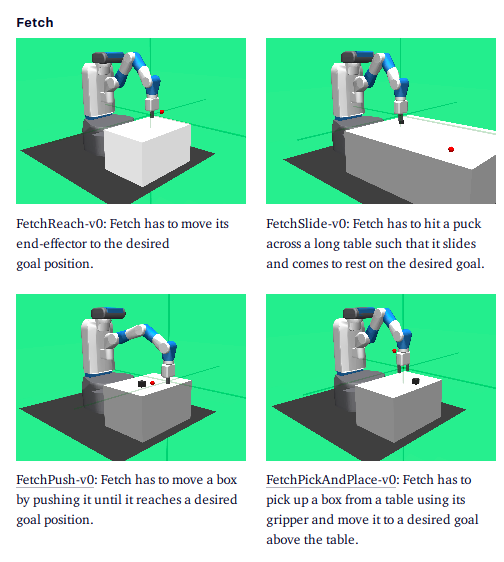
\includegraphics[height=0.8\textheight]{fetch.png}
        \caption{The Fetch environment (source: \href{https://www.cnblogs.com/siahekai/p/14161023.html}{cnblogs}).}
    \end{figure}
\end{frame}

\begin{frame}{Action Space}
    \vfill
    \begin{itemize}
        \item An action represents the Cartesian displacement dx, dy, and dz of the end effector.
        \item For some tasks, there is also a last action that controls closing and opening of the gripper.
    \end{itemize}
    \vfill
    \begin{tabular}{|l|c|c|c|}
        \hline
        Action & Control Min & Control Max & Unit \\
        \hline
        Displacement of the end effector in the x direction & -1 & 1 & position (m) \\
        \hline
        Displacement of the end effector in the y direction & -1 & 1 & position (m) \\
        \hline
        Displacement of the end effector in the z direction & -1 & 1 & position (m) \\
        \hline
    \end{tabular}
    \vfill
\end{frame}

\begin{frame}{State Space (FetchReach)}
    \vfill
    \begin{itemize}
        \item The observation space consists of information about the robot's end effector state and goal.
        \item Unlike the actions, the observations can take any value in $\mathbb{R}$.
    \end{itemize}
    \vfill
    \begin{tabular}{|l|c|}
        \hline
        Observation & Unit \\
        \hline
        Position of the end effector & position (m) \\
        \hline
        Joint displacement of the left and right gripper finger & position (m) \\
        \hline
        Linear velocity of the end effector & velocity (m/s) \\
        \hline
        Linear velocity of the left and right gripper finger & velocity (m/s) \\
        \hline
        Final goal position of the end effector & position (m) \\
        \hline
    \end{tabular}
    \vfill
\end{frame}

\begin{frame}{State Space (FetchPush)}
    \begin{tabular}{|l|c|}
        \hline
        Observation & Unit \\
        \hline
        Position of the end effector & position (m) \\
        \hline
        Joint displacement of the left and right gripper finger & position (m) \\
        \hline
        Linear velocity of the end effector & velocity (m/s) \\
        \hline
        Linear velocity of the left and right gripper finger & velocity (m/s) \\
        \hline
        Position of the block & position (m) \\
        \hline
        Relative block position with respect to the gripper & position (m) \\
        \hline
        Global rotation of the block in a XYZ Euler frame rotation & angle (rad) \\
        \hline
        Relative block linear velocity with respect to the gripper & velocity (m/s) \\
        \hline
        Angular velocity of the block & angular velocity (rad/s) \\
        \hline
        Final goal position of the block & position (m) \\
        \hline
    \end{tabular}
\end{frame}

\begin{frame}{Other Details of the Environment}
    \begin{itemize}
        \item The goal is reached if the Euclidean distance between the desired goal and achieved position is lower than 0.05 m.
        \item The reward can be `sparse' (0 or -1) or `dense' (negative Euclidean distance between the achieved position and the desired goal).
        \item The initial position of the gripper and the base of the robot fixed at $(x,y,z) = [1.34, 0.75, 0.56] m$ and $(x,y,z) = [0.40, 0.48, 0] m$ respectively.
        \item The orientation (in quaternions) of the gripper and the block is initialized to $(w,x,y,z) = [1.0, 0.0, 1.0, 0.0]$.
        \item The initial and the target position of the block is set at an offset to the gripper's initial position. The offset is sampled from a uniform distribution with a range of $[-0.15, 0.15] m$.
    \end{itemize}
\end{frame}
